\section{Experimental Results}
\subsection{Calibrating threshold values}
\label{sec:calibrate}

Simply configuring the PowerDue and FXOS8700CQ with interrupts would not work
because there is continuous variation in the magnetic field of a local
environment, and hence the sensor would continuously detect magnetic events and
send interrupts. To make the interrupts more useful, FXOS8700CQ can be
configured to only interrupt when the mangetic readings from any of the axes
cross a threshold value \cite{DatasheetSPI}. To compute $x_{th}$, $y_{th}$, and
$z_{th}$, we added a multiple of the standard deviation of the readings to the
absolute value of the mean of the readings. We experimented with different
values of the standard deviation multiplier, $m$, and concluded that $m = 8$
resulted in an adequate sensitivity level for our use case, mainly being able to
detect magnetic events caused by moving a cell phone, or magnetic strip, close
to the sensor.

Essentially, calibration allows us to treat the average values of the readings
due to magnetic variation as zero, as if we were translating the offset value of
the axes. FXOS8700CQ  provides offset registers which can be applied to the
readings after an event has been detected \cite{DatasheetSPI}, and hence this is
something that can be used to avoid having to manually translate values.

\subsection{Enabling interrupts on PowerDue}
\label{sec:powerdue_int}

To enable interrupts on the PowerDue, an interrupt handler has to be registered
with \textit{attachInterrupt} \cite{InterruptRef}, and the interrupt pin has to
be configured as an input pin. FXOS8700CQ can be configured to make the
interrupt signal active high or active low, but we found the default setting to
be active low, and hence configured the interrupt handler for this. Furthermore,
we found it useful to detach the interrupt handler after receiving an interrupt
signal, and to not reattach it until the magnetic event had been completely
processed by the application, which in this case meant until
\textit{ProcessData}, a task for counting the number of events detected, had
finished incrementing the counter for the number of events detected.

%\begin{figure}[h]
%\centering
%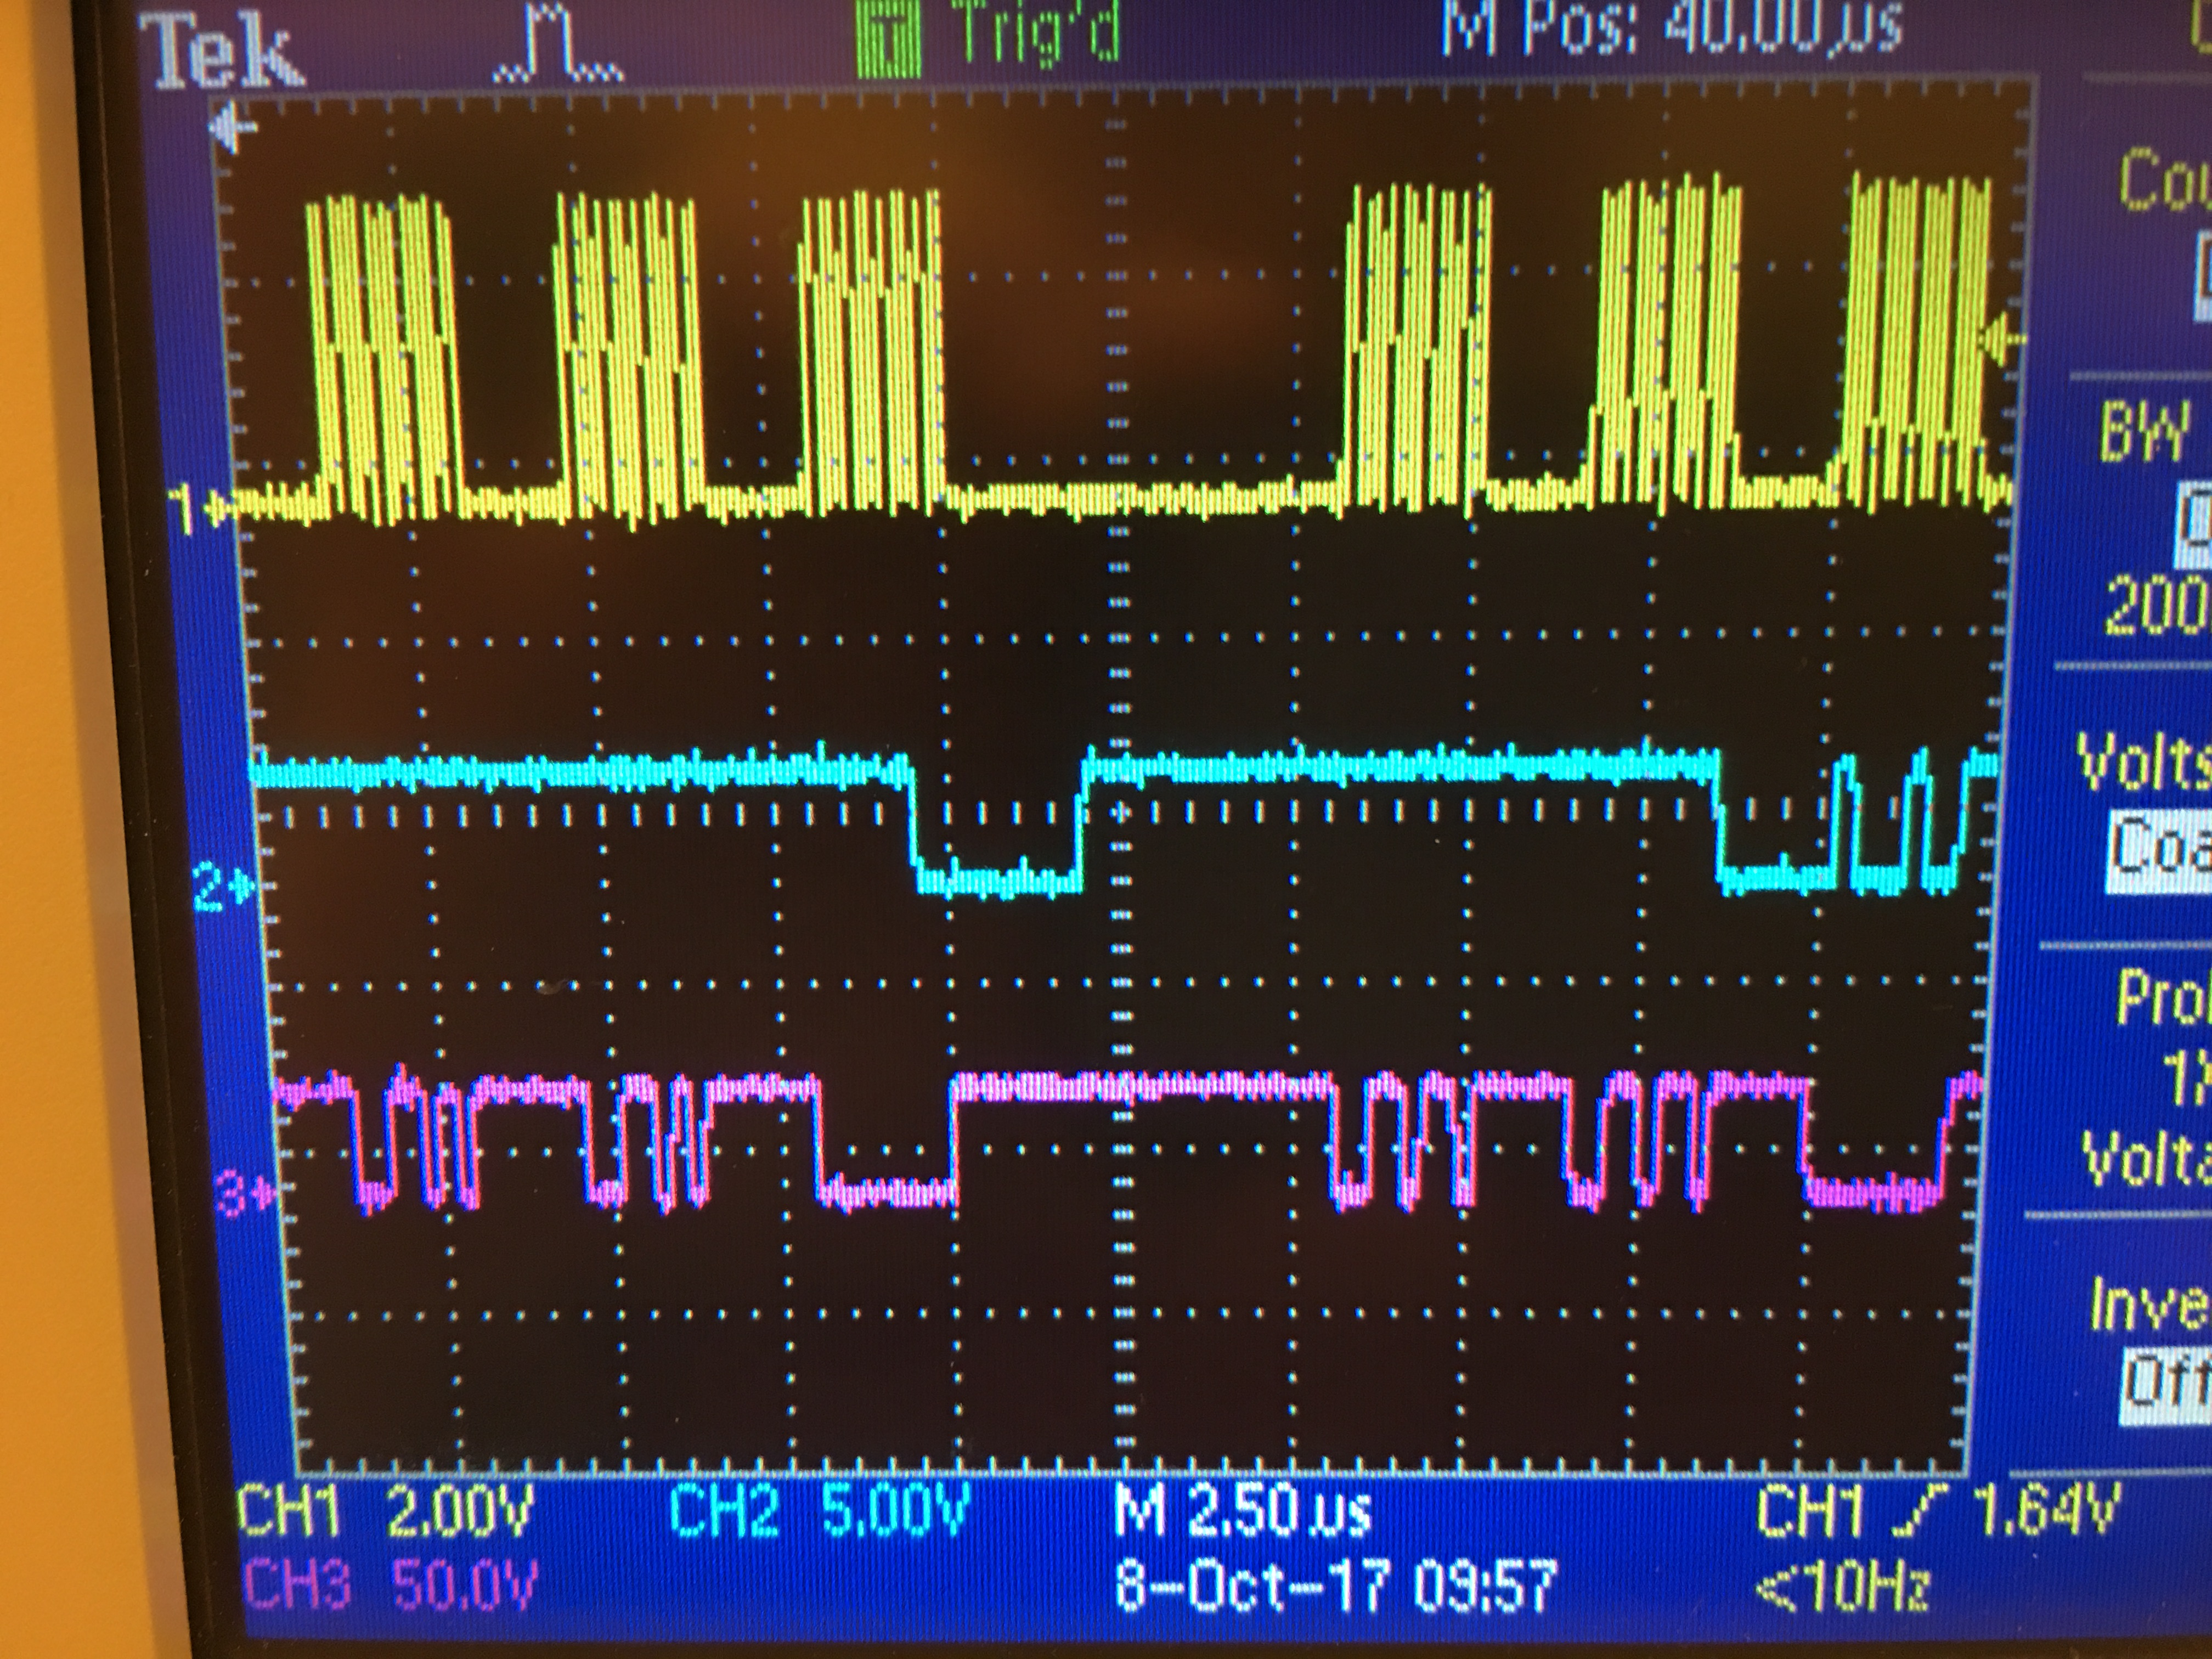
\includegraphics[width=0.4\textwidth]{spi_oscilloscope}
%\caption{SPI reads for the magnetometer data}
%\label{fig:spiOscillo}
%\end{figure}


\subsection{Interrupts on FXOS8700CQ}
\label{sec:sensor_int}

To enable the FXOS8700CQ sensor to interrupt the PowerDue when it detected
mangetic events the threshold values, we had to configure the threshold register
\cite{DatasheetSPI} with the threshold events and the interrupt pin. It was also
necessary to add functionality to the FXOS8700CQ class representing the sensor,
functionality that would allow us to check that an event had indeed occurred,
and also verify that the values had crossed the threshold.

Without verifying that an event had occured, we would get spurios interrupts,
especially during initialization of the program. More specifically, we would get
one interrupt signal when the interrupt handler was initially registered,
despite the fact that no event had been detected. Thus, to check whether an
event had been detected, we would read the event detected bit in the M\_THS\_SRC
register \cite{DatasheetSPI}.

Looking at the event flag in M\_THS\_SRC did not completely prevent us from
reporting values that were not above the threshold, because the sensor
might update the magnetic values in between the event detection and when we
reported the values. To prevent this from happening, we would only report the
values if we confirmed that they were above the threshold.

For our use case, it was also useful to add a delay of 1 second after processing
an event. Adding the delay allowed us to more intuitively associate an event
with a reported value, and in our case an event meant moving a cell phone or
magnetic strip close to the sensor. Without the delay, the application would
report a burst of events, making it seem like there had been multiple events
(indeed, it is logical to expect this, but we simply wanted to associate one
reported value to an event, and this made it easier to do so).
